\chapter{Quickstart}\label{cha:quickstart}

This chapter provides instructions for using XCSoar in typical
cross-country tasks.  It is separated into simple scenarios to
demonstrate how to use key features.  It assumes the configuration
options have already been set up to the user's preferences.

These instructions are intended to provide a simple step-by-step guide
to flying tasks of varying levels of complexity but are not intended
to demonstrate all the features of XCSoar.  Furthermore, the system
can be used productively in ways other than as described here.

\section{Local flight}\label{sec:local-flight}

In this scenario, the pilot intends to fly locally or a casual
cross-country task where navigation to pre-determined waypoints is not
required.

\subsection*{Prior to takeoff}
\begin{enumerate}
\item  Turn on the device.
\item  Open the \button{Flight Setup} dialog and adjust the bugs and ballast as
required. Set the maximum forecast temperature.  Close the dialog.
\item  Open the \button{Task Edit} dialog, and create a blank task by pressing
\button{New}.
\item  Select ``Touring'' as  task type.
\item  Once the task is created, move the cursor to the ``add waypoint'' item
and press enter.  Select the start waypoint from the list, e.g. first item is the home base, and press enter.
Press close or escape.
\item Select another one ``add waypoint'', and enter th same waypoint as finsh
point.
\item  Now the task contains one waypoint to home.
\end{enumerate}

\subsection*{In-flight}
\begin{enumerate}
\item  At the appropriate times, set the MacCready manually from the menu,
  task calculator or from the variometer.
\item  Change the bugs/ballast settings as required.
\item  At any time, the glider can reach home when the altitude difference
  bar is a green arrow pointing upwards.
\item  Optionally, activate \button{MC Auto} when ready to return
home. If the MacCready mode was set to ``Final Glide'' or ``Both'', then the
system will command the optimal speed to return home.
\end{enumerate}

\subsection*{After landing}
\begin{enumerate}
\item  The \button{Status} dialog shows the elapsed flight time.
\item  The analysis dialog can be used to analyse or review the flight.
\item  The IGC logger replay can be used to replay the flight.
\item  These actions may be performed after turning the device off and 
  on again. 
\end{enumerate}

\section{FAI Task}\label{sec:fai-task}

In this scenario, the pilot intends to fly a triangle FAI task with a
single start sector and automatic waypoint advance.

\subsection*{Prior to takeoff}
\begin{enumerate}
\item  Turn on the device.
\item  Open the \button{Flight Setup} dialog and adjust the bugs and ballast as
required. Set the maximum forecast temperature.  Close the dialog.
\item  Open the \button{Task Edit} dialog, and create a blank task by pressing
\button{New}. Select ``FAI triangle'' as task type.
\item  Move the cursor to the ``add waypoint'' item and press enter.  Set the
start and sector type and select the desired waypoint from the list and press enter.  Once finished, press close.
\item  Move the cursor to the ``add waypoint'' item again and press enter. 
Select the waypoint from the list and press enter.  This will add the first waypoint to the task.
\item  Repeat the procedure for the second waypoint. A good idea to find the
right second turn is to filter the waypoint list by bearing (+120°) and the
proper distance of the triangles edge. The filter references to
the first waypoint of our trianlge.
\item  Repeat the last step as required for an additional waypoint.  The last
waypoint is the finish waypoint.
\item  The task is now entered.  You may declare it and send the task to a
connected logger device.
\end{enumerate}

\subsection*{In-flight}
\begin{enumerate}
\item  The current waypoint will advance automatically as the pilot flies
through the observation zones.  
\item  After the task is started, the \button{Status} dialog can be opened to
verify a valid start was detected.  ``Valid Start" should be tagged as true,
The start time can be reviewed, the start height is saved and the min. finish
hight according given rules is shown.
\item  At all times the black track arrow will point at the next waypoint.  The
blue arrow will point at the direction the glider should track when in cruise.
\item  If \button{Zoom Auto} is activated, the map will automatically zoom in as
task waypoints are approached.
\item  At the appropriate times, adjust the MacCready by the menu,
the task calculator or the connected variometer; or activate \button{MC Auto}.
If the MacCready mode was set to `Final Glide' or `Both', then the system will command the optimal 
speed to return home; and the MacCready value will be set to the minimum climb
rate at which it is beneficial to continue to climb.
\item  Change the bugs/ballast settings as required.
\item  Refer to the \button{Analysis} dialog as required. 
\item  Refer to the \button{Status} dialog as required.  This shows the start
time, elapsed time on task, estimated arrival time, average task speed etc.
\item  At any time, when the altitude difference bar is a green arrow pointing 
upwards the glider can finish the task.

\end{enumerate}

\subsection*{After landing}
As described in Section~\ref{sec:local-flight}.


\section{AAT Task, Manual Arm}\label{sec:aat-task-manual}

In this scenario, the pilot intends to fly a triangle AAT task, and
will manually arm the waypoint advance system.

\subsection*{Prior to takeoff}
\begin{enumerate}
\item  Turn on the device.
\item  Open the \button{Flight Setup} dialog and adjust the bugs and ballast as
required. Set the maximum forecast temperature.  Close the dialog.
\item Open the \button{Task Edit} dialog, and create a blank task by pressing
\button{New}. Select ``AAT'' as task type.
\item  Once the task is created, move the cursor to the `add waypoint' item
and press enter.  Add waypoints in the already described way. 
\item  The AAT requires additional input to the kind and size of the
obserservation zone. Adjust AAT sector parameters for this waypoint and press
close or escape.
\item  Repeat the last two steps as required for additional waypoints.  The last
waypoint is the finish waypoint.
\item  The AAT task is now entered.  Open the \button{Properties} dialog
and set the given task time. 
\item  The estimated elapsed time to complete the task with different MacCready
settings can be explored from the \button{Task Calc} dialog.  Adjusting the MacCready value and see what
``AAT Range'' setting is suggested by XCSoar.
\end{enumerate}

\subsection*{In-flight}
\begin{enumerate}
\item  When the pilot is ready to start the task, press the \button{Arm
Start} button.  The current waypoint will then advance automatically
once, as the pilot flies through the start sector.  After this occurs, the advance trigger is disarmed.  
\item  In order to re-start, the pilot needs to manually revert to the
\button{Start Turnpoint} and again press the \button{Arm Start} button prior to
flying through the start sector again.
\item  After the task is started, the \button{Status} dialog can be opened to
verify a valid start was detected. If the start time is given, the start was detected and legal according to 
the task start rules specified in the configuration.  Otherwise it will display ``INVALID''.
\item  During flight, the estimated elapsed time to complete the task with
different MacCready settings can be explored from the \button{Task Calc} dialog.
Once a decision is made to extend or reduce the AAT range this can be done by
manually manipulate the \button{Target}. This allows the pilot to effectively increase or decrease the task
distance and estimate the consequence in AAT time.

The figure below shows the course around the targets at range set to $-100$\%.
\begin{center}
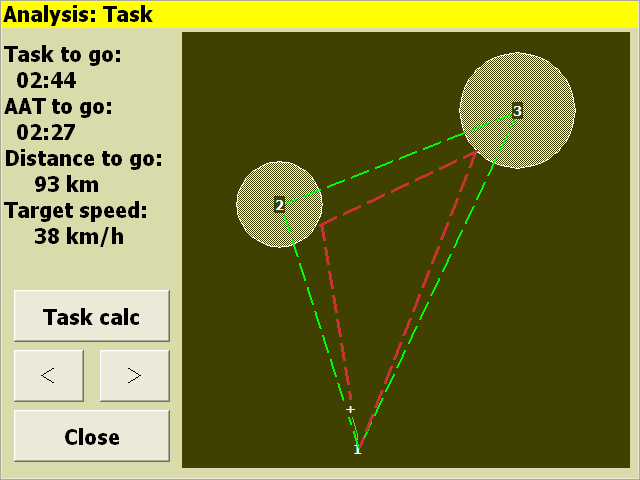
\includegraphics[angle=0,width=0.8\linewidth,keepaspectratio='true']{figures/aat-short.png}
\end{center}

The figure below shows the course around the targets at range set to $100$\%.
\begin{center}
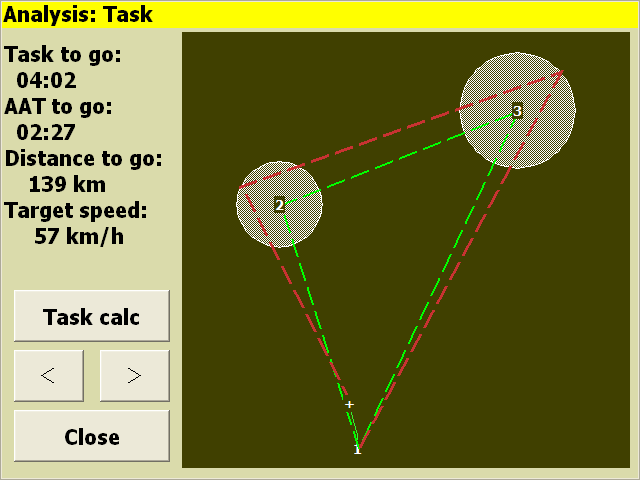
\includegraphics[angle=0,width=0.8\linewidth,keepaspectratio='true']{figures/aat-long.png}
\end{center}

\item  At all times the black track arrow will point at the next target.  The
target is the location within the AAT sector at the range specified in
the \button{Task Calc} dialog.  The blue arrow will point at the direction
the glider should track when in cruise.

\item  When the pilot is within or approaching an AAT sector and is ready to
advance to the next waypoint, press the \button{Arm Turn} button.  The
current waypoint will then advance automatically once, if the pilot is
inside the observation zone.  After this occurs, the advance trigger
is disarmed.

\item If Auto Zoom is activated, the map will automatically zoom in as task waypoints are approached.

\item  At the appropriate times, adjust the MacCready by the menu,
the task calculator or the connected variometer; or activate \button{MC Auto}.
If the MacCready mode was set to `Final Glide' or `Both', then the system will command the optimal 
speed to return home; and the MacCready value will be set to the minimum climb
rate at which it is beneficial to continue to climb.
  
\item  Change the bugs/ballast settings as required.
\item  Refer to the \button{Analysis} dialog as required. 
\item  Refer to the \button{Status} dialog as required.  This shows the start
time, elapsed time on task, estimated arrival time, average task speed etc.
\end{enumerate}

\subsection*{After landing}
As described in Section~\ref{sec:local-flight}.

% Agian in 6.1 
%\section{Task with alternate start sectors}
%
%In this scenario, the pilot intends to fly a task with 
%alternate start sectors and manually arm the waypoint advance system.
%
%\subsection*{Prior to takeoff}
%As described in Section~\ref{sec:fai-task}, except where noted below.
%\begin{enumerate}
%\item Open the `Task edit' dialog, and set `Auto Advance' to `Arm start'.
%  Select the start waypoint, and press enter.  Set `Alternate Start
%  Points' to ON, and press `Edit start points'.  Press `clear' to
%  clear the list of existing start points if required.  Move the
%  cursor to a blank line or `add waypoint' line and press enter; then
%  select the waypoint and press enter.  Repeat for each alternate
%  start point.
%\end{enumerate}
%
%\subsection*{In-flight}
%As described in Section~\ref{sec:fai-task}, except where noted below.
%\begin{enumerate}
%\item 
%Prior to entering the start sector, when the pilot is ready to start
%the task, press the `Arm Advance' button.
%
%\item 
%In order to re-start from any start sector, the pilot needs to press
%the `Arm Advance' button again prior to flying through any of the
%start sectors again.
%\end{enumerate}

